\documentclass[12pt]{article}
\usepackage{setspace, graphicx, fullpage, amssymb, amsmath, epsfig, natbib, array, multirow, hyperref}
\usepackage{amsfonts, bm} 
\usepackage{dcolumn}
\usepackage{subfigure, float} 
\usepackage[margin=1in]{geometry} 
\usepackage{verbatim}
\usepackage{url}
\usepackage{enumerate}
\usepackage{morefloats}
\usepackage{caption}
\newcolumntype{d}[1]{D{.}{.}{#1}} 

\newcommand\fnote[1]{\captionsetup{font=small}\caption*{#1}}

\begin{document}

\section{Overview}

At our previous meeting we decided to:

\begin{itemize}
	\item Consider alternative placebo tests to seniority
	
	\item Make additional improvements to prepare it for outside critique and reworking by William and Craig
\end{itemize}

\subsection{Alternative Placebo Tests}

If we are unhappy with the present use of higher seniority as a placebo test (given the fact that a higher seniority member will more often be nearer election or otherwise) we will need to select something else which would meaningfully separate same-state Senator pairs. Here I lay out a few additional possibilities:

The main alternative I can think of which would be related to reelection would be the number of votes cast in a particular Congress. A possible alternative mechanism would be that those up for reelection are not less responsive to the party because they are taking their constituents into greater account but instead because they are less present in Washington. Of course, this would also likely mean that they were spending more time in their state.

If we show this, we would only want to show the difference-in-differences, since the differences alone are not indicative of what we want to highlight:

\begin{figure}[H]
	\centering
	\caption{Senate Rate of Voting With Party by Vote Type}
	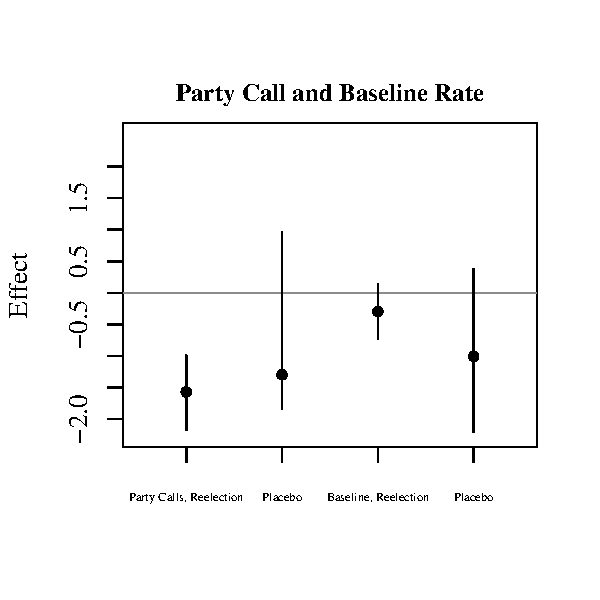
\includegraphics[width = 10cm]{C:/Users/Ethan/Documents/GitHub/partycalls/plots/senate-diff-coeff-vote-placebo.pdf}
	\fnote{\textit{Note}: The treatment in this test is being up for reelection while the placebo is having cast fewer votes than a same-state Senator when neither are up for reelection. In both the treatment and placebo tests, responsiveness to party calls and baseline rate of voting with the party is considered between same-state Senator pairs.}
\end{figure}

However, the changes are comparable across vote types in a way which is not seen in the reelection condition, so we could just show the difference-in-differences which is in line with our expectations:

\begin{figure}[H]
	\centering
	\caption{Senate Party Call Response Rate Difference from Baseline Rate of Voting with Party}
	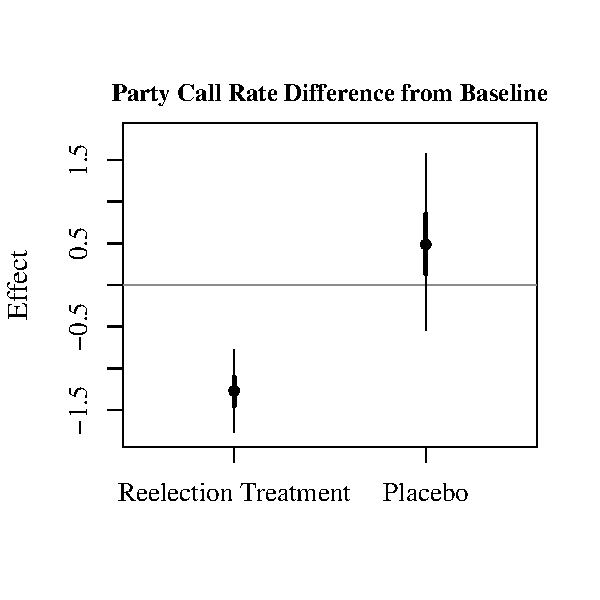
\includegraphics[width = 10cm]{C:/Users/Ethan/Documents/GitHub/partycalls/plots/senate_diff_in_diff_vote_placebo.pdf}
	\fnote{\textit{Note}: The treatment in this test is being up for reelection while the placebo is having cast fewer votes than a same-state Senator when neither are up for reelection. In both the treatment and placebo tests, the difference between the responsiveness to party calls and baseline rate of voting with the party is considered between same-state Senator pairs.}
\end{figure}

Alternatively, we could front-load the difference-in-differences and include the differences tests either in the paper or an appendix and explain that we see comparable changes in vote types for the less-often-voting Senator but that those up for reelection only change their stance on the party call votes.

\end{document}